\documentclass[12pt, a4paper]{article}

\usepackage[utf8]{inputenc}
\usepackage{mathptmx} % Times New Roman font
\usepackage{geometry}
\geometry{a4paper, margin=1in}
\usepackage{fancyhdr}
\setlength{\headheight}{15pt}
\usepackage{titlesec}
\usepackage{setspace}
\usepackage{graphicx}
\usepackage{listings}
\usepackage{tikz}
\usetikzlibrary{shapes.geometric, arrows, positioning, calc, fit, backgrounds}
\usepackage{float}
\usepackage{booktabs}
\usepackage{tabularx}
\usepackage{longtable}
\usepackage{hyperref}
\usepackage{array} % For advanced table column alignment
\usepackage[justification=centering, skip=10pt, font=rm]{caption} % Centered and uniformly formatted captions (Roman font)
\usepackage{parskip} % For paragraph spacing instead of indentation
\usepackage{chngcntr}
\usepackage{microtype} % Improves text alignment, spacing, and hyphenation
\usepackage{needspace}
\usepackage{placeins} % Dynamic space allocation to prevent orphan headings

% TikZ styles for custom flowcharts
\tikzstyle{process} = [rectangle, minimum width=4.5cm, minimum height=0.9cm, align=center, text width=4cm, draw=black, fill=blue!10, font=\normalsize\bfseries, inner sep=6pt, rounded corners=3pt]
\tikzstyle{groupbox} = [rectangle, draw=black!50, dashed, inner sep=8pt, fill=black!5, rounded corners]
\tikzstyle{arrow} = [thick,->,>=stealth]

% Table numbering includes section
\counterwithin{table}{section}

% Typographical Adjustments
\frenchspacing % Uniform spacing after periods (prevents large gaps)

% Uniform spacing around floats (Tables and Figures)
\setlength{\intextsep}{18pt}
\setlength{\textfloatsep}{18pt}

% Header and Footer Setup
\pagestyle{fancy}
\fancyhf{}
\fancyhead[R]{\rmfamily Urban Bike-Sharing Demand Forecasting Using Machine Learning}
\fancyfoot[L]{\rmfamily Department of Computer Applications}
\fancyfoot[R]{\rmfamily \thepage}
\renewcommand{\headrulewidth}{0.4pt}
\renewcommand{\footrulewidth}{0.4pt}

% Title Formatting (Ensuring consistent heading spacing and fonts)
\titleformat{\section}{\rmfamily\fontsize{16pt}{19.2pt}\selectfont\bfseries}{\thesection.}{0.3em}{}
\titleformat{\subsection}{\rmfamily\fontsize{14pt}{16.8pt}\selectfont\bfseries}{\thesubsection}{0.3em}{}
\titleformat{\subsubsection}{\rmfamily\fontsize{12pt}{14.4pt}\selectfont\bfseries}{\thesubsubsection}{0.3em}{}

% Line Spacing
\onehalfspacing

\raggedbottom % Prevents vertical stretching that causes unnatural gaps between paragraphs

\begin{document}
\pagenumbering{arabic}
\setcounter{page}{1}

% ==============================================================================
% 1. INTRODUCTION
% ==============================================================================
\section{Introduction}

Urban bike-sharing systems have emerged as one of the most promising and sustainable modes of public transportation in modern smart cities, offering an eco-friendly, cost-effective, and healthy alternative to fossil-fuel-dependent vehicles. By providing commuters with flexible point-to-point transit for first-mile and last-mile connectivity, bike-sharing networks mitigate vehicular traffic congestion, reduce carbon emissions, and promote active lifestyles. The integration of technology, mobile applications, and physical infrastructure has enabled these networks to expand rapidly worldwide. Over the past decade, these systems have evolved from simple coin-operated municipal programs into sophisticated, data-driven dockless and docked networks tracked continuously via GPS and cellular data arrays.

However, managing the operational equilibrium across a vast network of docking stations remains a profoundly complex logistical challenge. Because users do not return bicycles to their original starting locations, the system naturally flows out of balance. Unpredictable demand fluctuations frequently cause popular pickup stations (such as residential zones during the morning commute) to experience bicycle deficits (shortages), leaving intending users stranded. Conversely, popular destination hubs (such as commercial districts and major transit terminals) simultaneously reach full capacity and cannot accept incoming returns, causing massive surpluses. This imbalance creates a logistical nightmare for municipal operators who must deploy fleets of physical redistribution trucks to manually move bicycles back to where they are needed.

Advances in data-driven techniques and predictive analytics have established supervised machine learning as an effective and scalable solution for urban mobility forecasting. Machine learning models possess the capability to uncover complex, non-linear relationships between station usage patterns and a multitude of temporal factors, including peak commuting hours, day of the week, and seasonal shifts, without relying on rigid, static schedules. Traditional statistical models, such as Auto-Regressive Integrated Moving Average (ARIMA), often struggle to capture the high-frequency volatility of micro-mobility data, particularly when attempting to model dozens of independent stations simultaneously. In contrast, modern ensemble regression algorithms such as Random Forest, Extreme Gradient Boosting (XGBoost), and CatBoost are remarkably well-suited for capturing these intricate dynamics due to their exceptional predictive accuracy, non-linear mapping capabilities, and resilience against noisy transactional data.

This project focuses on building a comprehensive, intelligent machine learning pipeline to accurately forecast hourly bike-sharing departure demand across the San Francisco Bay Area network using extensive historical trip data. The target variable is explicitly defined as the hourly station-level departure demand, representing the exact number of trips starting from a particular station during a specific hour. This definition provides a direct, actionable metric for fleet operators. The historical dataset encompasses hundreds of thousands of individual bicycle trips across multiple urban cities, including San Francisco, San Jose, Mountain View, and Palo Alto. The end-to-end workflow involves systematic data preprocessing, chronological train-validation-test partitioning, advanced time-series feature engineering, and rigorous multi-model benchmarking.

Accurate bike-sharing demand forecasting directly enhances urban micro-mobility management in several profound ways. Primarily, it provides demand-based redistribution support, enabling transit operators to preemptively anticipate station deficits and allocate bicycles more efficiently before shortages occur. Furthermore, it improves overall commuter satisfaction by ensuring asset availability and minimizes the operational overhead associated with reactive vehicle dispatching. By combining historical trip records with state-of-the-art machine learning algorithms, this project delivers a reliable, scalable, and data-driven approach for smart city transit optimization, demonstrating how predictive analytics can transform physical infrastructure management.

In summary, the work aims to demonstrate the capability of supervised machine learning algorithms to forecast future demand using purely historical transactional data and rigorously evaluate predictive performance, thereby contributing significantly to the efficient operation and sustainability of modern urban transportation networks.


% ==============================================================================
% 2. SUPPORTING LITERATURE
% ==============================================================================
\section{Supporting Literature}
\subsection{Literature Review}

\begin{table}[H]
\centering
\renewcommand{\arraystretch}{1.5}
\begin{tabular}{|p{0.3\textwidth}|p{0.6\textwidth}|}
\hline
\textbf{TITLE} & Prediction bike-sharing demand with gradient boosting methods \\ \hline
\textbf{AREA OF WORK} & The paper focuses on applying machine learning and gradient boosting algorithms to predict bike-sharing demand across multiple urban environments (Konya and Washington D.C.) to optimize fleet distribution. \\ \hline
\textbf{DATASET} & Historical bike-sharing trip data from Konya, Turkey and Washington, D.C., USA, including meteorological parameters and temporal variables. \\ \hline
\textbf{METHODOLOGY /}\newline \textbf{STRATEGY} & The study uses historical data for training and testing. Data preprocessing involves extracting temporal features. Three gradient boosting algorithms are trained and evaluated using error metrics. \\ \hline
\textbf{ALGORITHM} & 
Extreme Gradient Boosting (XGBoost), Light Gradient Boosting Machine (LightGBM), CatBoost \\ \hline
\textbf{RESULT/PRECISION} & 
Gradient boosting methods demonstrated high resilience to noise and cyclical data. \\ \hline
\textbf{ADVANTAGES} & The study reports that gradient boosting handles non-linear temporal data effectively. \\ \hline
\textbf{FUTURE PROPOSAL} & Future research will explore real-time streaming data integration and hybrid deep learning models. \\ \hline
\end{tabular}
\caption{Literature Review: Prediction bike-sharing demand with gradient boosting methods}
\end{table}

\begin{table}[H]
\centering
\renewcommand{\arraystretch}{1.5}
\begin{tabular}{|p{0.3\textwidth}|p{0.6\textwidth}|}
\hline
\textbf{TITLE} & A predictive analytics approach for forecasting bike rental demand \\ \hline
\textbf{AREA OF WORK} & The paper focuses on evaluating the performance of six diverse machine learning regression models in forecasting hourly bike rental demand to improve operational balancing. \\ \hline
\textbf{DATASET} & Public bike rental records encompassing temporal features, weather conditions, and holiday indicators. \\ \hline
\textbf{METHODOLOGY /}\newline \textbf{STRATEGY} & Historical data was preprocessed and split into training and testing sets. Six different regression models were trained. Performance was compared using R-squared, RMSE, and MAE. \\ \hline
\textbf{ALGORITHM} & 
Ordinary Least Squares (OLS), Multi-Layer Perceptron (MLP), Gradient Boosting Regression, Random Forest Regression, Decision Tree Regression \\ \hline
\textbf{RESULT/PRECISION} & Random Forest and Gradient Boosting achieved the highest performance, heavily outperforming Neural Networks on tabular data. \\ \hline
\textbf{ADVANTAGES} & The paper provides a comparative analysis, highlighting the usefulness of tree-based bagging and boosting for mobility forecasting. \\ \hline
\textbf{FUTURE PROPOSAL} & Expanding the models to include dynamic pricing variables and weather forecasting integration. \\ \hline
\end{tabular}
\caption{Literature Review: A predictive analytics approach for forecasting bike rental demand}
\end{table}

\begin{table}[H]
\centering
\renewcommand{\arraystretch}{1.5}
\begin{tabular}{|p{0.3\textwidth}|p{0.6\textwidth}|}
\hline
\textbf{TITLE} & GSTGAT: Gated spatiotemporal graph attention network for traffic demand forecasting \\ \hline
\textbf{AREA OF WORK} & The paper focuses on predicting traffic and bike-sharing demand using complex deep learning graph architectures to capture spatial dependencies between stations. \\ \hline
\textbf{DATASET} & San Francisco Bay Area bicycle dataset (the same foundation utilized in this project). \\ \hline
\textbf{METHODOLOGY /}\newline \textbf{STRATEGY} & The study applied advanced graph attention mechanisms and gated recurrent units to model the network topology. Performance was evaluated against baseline deep learning models. \\ \hline
\textbf{ALGORITHM} & 
Yao et al. proposed GSTGAT, a spatiotemporal graph attention model that captures temporal and spatial relationships in traffic demand. The study includes the San Francisco Bay Area bicycle dataset. \\ \hline
\textbf{RESULT/PRECISION} & The model successfully captured spatial dependencies. \\ \hline
\textbf{ADVANTAGES} & Deeply models spatial topology, providing insight into how neighboring stations influence each other. \\ \hline
\textbf{FUTURE PROPOSAL} & Exploring hybrid architectures that combine tree-based tabular models with spatial graph embeddings. \\ \hline
\end{tabular}
\caption{Literature Review: GSTGAT for traffic demand forecasting}
\end{table}

\subsection{Literature Review Summary}

\begin{table}[H]
\centering
\renewcommand{\arraystretch}{1.5}
\begin{tabular}{|p{0.3\textwidth}|p{0.6\textwidth}|}
\hline
\textbf{TITLE} & \textbf{SUMMARY} \\ \hline
\textbf{Paper 1: Prediction bike-sharing demand with gradient boosting methods} & This study evaluates predicting bike-sharing demand using XGBoost, LightGBM, and CatBoost across two distinct cities. It shows that gradient boosting frameworks are exceptionally capable of capturing cyclical human mobility patterns. \\ \hline
\textbf{Paper 2: A predictive analytics approach for forecasting bike rental demand} & This work compared six models (Random Forest, MLP, OLS, Decision Trees) for rental demand forecasting. The results highlighted that ensemble tree methods heavily outperformed standard neural networks on tabular data, providing a stable and generalizable solution. \\ \hline
\textbf{Paper 3: GSTGAT: Gated spatiotemporal graph attention network} & This study utilized the SF Bay Area dataset to build a graph neural network. Yao et al. proposed GSTGAT, a spatiotemporal graph attention model that captures temporal and spatial relationships in traffic demand. \\ \hline
\end{tabular}
\caption{Literature Review Summary}
\end{table}

\subsection{Findings and Proposals}
The initial study reviewed by Aydın et al. (2023) examined the prediction of bike-sharing demand using advanced gradient boosting. The primary takeaway from this research is that integrating sequential error-correcting algorithms like XGBoost and CatBoost improves the reliability of forecasting, making it more applicable for practical uses such as managing fleet distribution.

The second study by Karunanithi et al. (2024) presented a comparative analysis of machine learning predictive models. The study found strong performance from tree-based ensemble methods for bike rental demand forecasting.

The third research effort by Yao et al. (2024) evaluated the effectiveness of deep learning structures. Yao et al. proposed GSTGAT, a spatiotemporal graph attention model that captures temporal and spatial relationships in traffic demand. The study includes the San Francisco Bay Area bicycle dataset.


% ==============================================================================
% 3. SYSTEM ANALYSIS
% ==============================================================================
\section{System Analysis}

\subsection{Analysis of the dataset}
This section provides a detailed analysis of the dataset utilized for training and evaluating the predictive models. The raw transactional records undergo a systematic examination to understand their structure and distribution.
\subsubsection{About the dataset}
\textbf{a) Dataset Overview}

The foundation of this predictive modeling project is the SF Bay Area Bike Share Dataset. To ensure the model relies strictly on historically verified, transactional human behavior rather than external approximations, the final implementation uses exclusively the \texttt{trip.csv} file from the dataset.

\begin{itemize}
    \item \textbf{Total Raw Records:} 669,959 individual, anonymized bicycle trip transactions.
    \item \textbf{Time Span:} The dataset covers the period from 29 August 2013 to 31 August 2015.
    \item \textbf{Total Features:} 12 raw columns.
    \item \textbf{Data Types:} A mix of numerical IDs, integers, and string objects (which must be converted to datetime).
    \item \textbf{Target Variable:} \texttt{hourly\_demand} (calculated by aggregating \texttt{start\_date} and \texttt{start\_\allowbreak station\_\allowbreak id}).
\end{itemize}

The overall workflow is presented in Figure~\ref{fig:project_workflow}.

\clearpage
\textbf{b) Dataset sample records}

\begin{figure}[H]
\centering
\includegraphics[width=0.9\textwidth]{fig_3_1_shape_dtypes.png}
\caption{Result of shape and datatype of dataset}
\label{fig:shape_dtypes}

\end{figure}

This figure displays the programmatic output verifying the fundamental structure of the imported dataset. It confirms that the data matrix contains exactly 669,959 rows and 12 columns. Furthermore, it details the memory datatypes assigned to each column.


\needspace{12\baselineskip}
\subsubsection{Explore the dataset}

\begin{figure}[H]
\centering
\includegraphics[width=0.9\textwidth]{fig_3_3_first_10_records.png}
\caption{First ten records of the dataset}
\label{fig:first_10_records}

\end{figure}

This screenshot provides a direct glimpse into the raw transactional data structure by displaying the top 10 rows. It illustrates exactly how a single trip is recorded: showing the trip ID, duration, timestamp, and station details.


\begin{figure}[H]
\centering
\includegraphics[width=0.9\textwidth]{fig_3_4_summary_stats.png}
\caption{Summary Statistics of Numeric Columns}
\label{fig:summary_stats}

\end{figure}

The summary statistics table provides mathematical insights into the distribution of the numerical columns. Crucially, by examining the \texttt{duration} column, we can observe the presence of massive outliers, justifying our architectural decision to forecast sheer departure volume rather than attempting to predict trip duration.


\needspace{12\baselineskip}
\subsection{Data Preprocessing}
\subsubsection{Data Cleaning}

\begin{figure}[H]
\centering

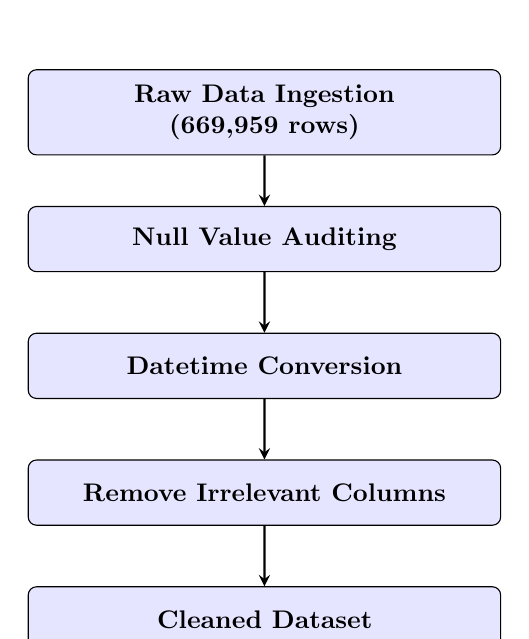
\begin{tikzpicture}[node distance=1.75cm, auto, scale=0.92, every node/.style={transform shape}]
    \tikzstyle{dcprocess} = [rectangle, minimum width=6.5cm, minimum height=0.9cm, align=center, text width=6.1cm, draw=black, fill=blue!10, font=\normalsize\bfseries, inner sep=6pt, rounded corners=3pt]
    \node [dcprocess] (step1) {Raw Data Ingestion\\(669,959 rows)};
    \node [dcprocess, below of=step1] (step2) {Null Value Auditing};
    \node [dcprocess, below of=step2] (step3) {Datetime Conversion};
    \node [dcprocess, below of=step3] (step4) {Remove \mbox{Irrelevant} Columns};
    \node [dcprocess, below of=step4] (step5) {Cleaned Dataset};
    
    \draw [arrow] (step1) -- (step2);
    \draw [arrow] (step2) -- (step3);
    \draw [arrow] (step3) -- (step4);
    \draw [arrow] (step4) -- (step5);
\end{tikzpicture}
\caption{Detailed Data Preprocessing Flow}
\label{fig:preprocessing_flow}

\end{figure}

This flowchart illustrates the sequential steps taken during the data cleaning phase:
\begin{itemize}
    \item \textbf{Step 1 -- Raw Data Ingestion (669,959 rows):} Ingest the raw transaction records from \texttt{trip.csv}, comprising 669,959 individual bicycle rental records collected across the regional network.
    \item \textbf{Step 2 -- Null Value Auditing:} Programmatically audit all columns for missing, corrupt, or unrecorded entries to guarantee complete data integrity across routing variables.
    \item \textbf{Step 3 -- Datetime Conversion:} Parse string timestamp fields into standardized pandas datetime objects to enable granular temporal filtering and time-series feature extraction.
    \item \textbf{Step 4 -- Remove Irrelevant Columns:} Remove non-predictive attributes (e.g., zip code and subscriber metadata) to eliminate noise and optimize memory consumption.
    \item \textbf{Step 5 -- Cleaned Dataset Output:} Export a structurally verified dataset containing valid departure records, establishing the foundation for station-hour grid construction.
\end{itemize}


\begin{figure}[H]
\centering
\includegraphics[width=0.9\textwidth]{fig_3_11_missing_values.png}
\caption{Missing Values Verification}
\label{fig:missing_values}

\end{figure}

This figure displays the result of the null-value checking algorithm. It verifies the operational integrity by proving that zero records are missing critical routing data.


\begin{figure}[H]
\centering
\includegraphics[width=0.9\textwidth]{fig_3_14_outliers.png}
\caption{Outlier Detection and Handling}
\label{fig:outliers}

\end{figure}

This visualization illustrates the identification and handling of anomalous or extreme trip-duration values during the data cleaning phase.


\needspace{12\baselineskip}
\subsubsection{Analysis of Feature Variables}

\begin{figure}[H]
\centering

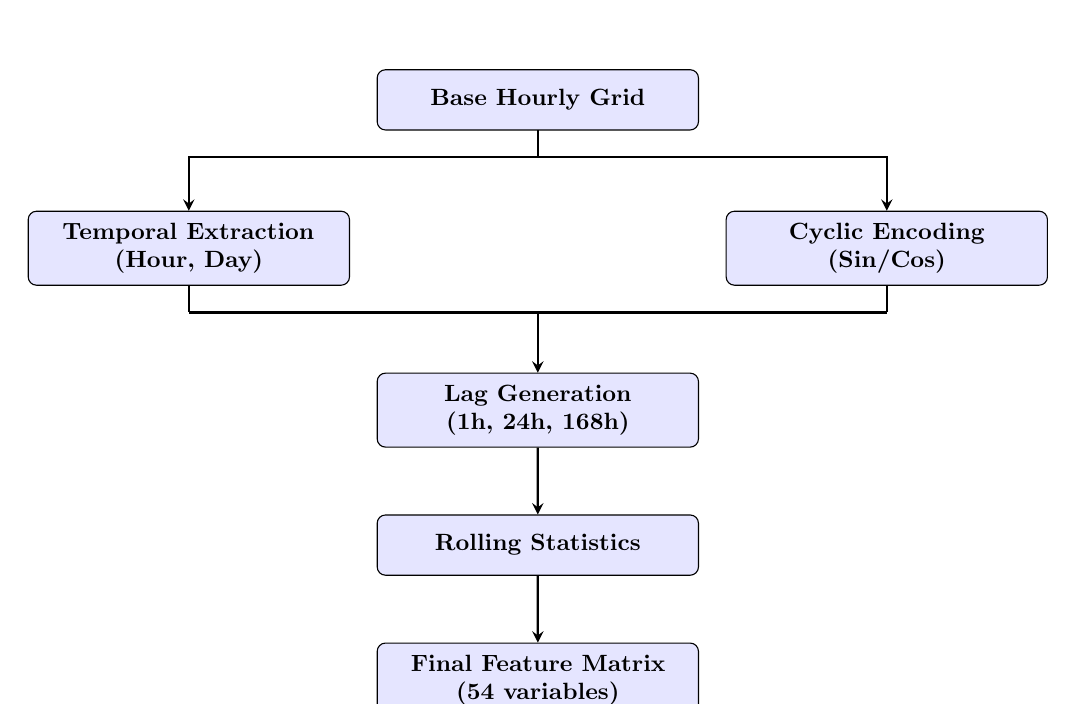
\begin{tikzpicture}[auto, scale=0.85, every node/.style={transform shape}]
    \tikzstyle{feprocess} = [rectangle, minimum width=4.8cm, minimum height=0.9cm, align=center, text width=4.4cm, draw=black, fill=blue!10, font=\normalsize\bfseries, inner sep=5pt, rounded corners=3pt]
    
    \node [feprocess] (step1) {Base Hourly Grid};
    \node [feprocess, below left=1.2cm and 0.4cm of step1] (step2a) {Temporal Extraction\\(Hour, Day)};
    \node [feprocess, below right=1.2cm and 0.4cm of step1] (step2b) {Cyclic Encoding\\(Sin/Cos)};
    
    \node [feprocess, below=1.3cm of $(step2a.south)!0.5!(step2b.south)$] (step3) {Lag Generation\\(1h, 24h, 168h)};
    \node [feprocess, below=1.0cm of step3] (step4) {Rolling Statistics};
    \node [feprocess, below=1.0cm of step4] (step5) {Final Feature Matrix\\(54 variables)};
    
    % Split from Base Grid to Temporal & Cyclic
    \draw [thick] (step1.south) -- ++(0,-0.4) coordinate (split);
    \draw [arrow] (split) -| (step2a.north);
    \draw [arrow] (split) -| (step2b.north);
    
    % Join from Temporal & Cyclic into Lag Generation
    \draw [thick] (step2a.south) -- ++(0,-0.4) coordinate (join1);
    \draw [thick] (step2b.south) -- ++(0,-0.4) coordinate (join2);
    \draw [thick] (join1) -- (join2);
    \coordinate (join_mid) at ($(join1)!0.5!(join2)$);
    \draw [arrow] (join_mid) -- (step3.north);
    
    % Downward pipeline
    \draw [arrow] (step3) -- (step4);
    \draw [arrow] (step4) -- (step5);
\end{tikzpicture}
\caption{Feature Engineering Pipeline}
\label{fig:fe_flow}

\end{figure}

This diagram breaks down the specific feature engineering operations applied to the dataset:
\begin{itemize}
    \item \textbf{Step 1 -- Base Hourly Grid Construction:} Construct a complete Cartesian grid crossing all 70 docking stations with all 17,583 continuous chronological hours ($1,230,810$ records), explicitly populating hours without departures with a count of zero.
    \item \textbf{Step 2 -- Temporal Extraction (Hour, Day):} Extract fundamental calendar features directly from the timestamp, including hour of day (0--23), day of week (0--6), month, and a binary indicator separating weekdays from weekends.
    \item \textbf{Step 3 -- Cyclic Encoding (Sin/Cos):} Apply trigonometric sine and cosine transformations ($\sin(2\pi t/T)$ and $\cos(2\pi t/T)$) to 24-hour and 7-day cycles to mathematically reflect periodic temporal continuity across midnight and week boundaries.
    \item \textbf{Step 4 -- Lag Generation (1h, 24h, 168h):} Generate historical demand lag features at 1-hour ($t-1$), 24-hour ($t-24$, previous day), and 168-hour ($t-168$, previous week) intervals to provide the models with critical recent and cyclical demand baselines.
    \item \textbf{Step 5 -- Rolling Statistics:} Compute backward-looking multi-hour rolling window statistics across the station-hour grid, including rolling mean, maximum, minimum, standard deviation, and median features over multiple historical time windows to capture short-term demand trends and local volatility.
    \item \textbf{Step 6 -- Final Feature Matrix (54 variables):} Consolidate all engineered temporal, cyclical, lag, and rolling predictors into the finalized 54-feature matrix, strictly audited against target leakage.
\end{itemize}

To transform the raw transactional records into a format suitable for machine learning, a complete Cartesian grid comprising all 70 stations and all 17,583 hourly timestamps was constructed. Zero-demand hours were appropriately filled with 0. 54 distinct numerical features were engineered.

\begin{figure}[H]
\centering
\includegraphics[width=0.9\textwidth]{fig_3_15_cyclic.png}
\caption{Handling Cyclic Features Implementation}
\label{fig:cyclic_features}

\end{figure}

This figure demonstrates the Python implementation of the trigonometric cyclic encoding process for time variables.


\begin{figure}[H]
\centering
\includegraphics[width=0.9\textwidth]{fig_3_19_vif.png}
\caption{Variance Inflation Factor (VIF) Analysis}
\label{fig:vif}

\end{figure}

This feature engineering diagnostic tests for multi-collinearity among the 54 engineered predictors.


\subsubsection{Analysis of Class Variables}
The target variable is the hourly station-level departure demand. This represents the absolute count of bicycle trips starting from a specific docking station during a specific one-hour block.

\begin{itemize}\setlength{\itemsep}{1pt}\setlength{\parskip}{0pt}
    \item Mean Demand: 0.5443
    \item Standard Deviation: 1.5453
    \item Maximum Demand: 52
    \item Zero-demand records: 946,161
    \item Positive-demand records: 284,649
\end{itemize}

This is a regression target, not a categorical class variable.

\subsection{Data Visualization}

\begin{figure}[H]
\centering
\includegraphics[width=0.90\textwidth]{hourly_demand.png}
\caption{Hourly Demand Pattern Across All Stations}
\label{fig:hourly_demand}

\end{figure}

This plot displays the aggregate hourly demand pattern across all stations in the network, revealing a clear bimodal distribution indicative of commuter behavior.


\begin{figure}[H]
\centering
\includegraphics[width=0.80\textwidth]{weekday_demand.png}
\caption{Demand Pattern Based on Day of the Week}
\label{fig:weekday_demand}

\end{figure}

This bar chart compares overall departure volumes by day of the week, clearly demonstrating that weekday usage heavily outpaces weekend usage due to regular commuting.


The analysis shows substantially higher weekday demand than weekend demand. This indicates that day-of-week information is useful for demand forecasting.

\begin{figure}[H]
\centering
\includegraphics[width=0.80\textwidth]{top20_stations.png}
\caption{Top 20 Busiest Docking Stations}
\label{fig:top_stations}

\end{figure}

\clearpage
This figure identifies the top 20 busiest docking stations in the system, highlighting the disproportionate demand concentrated at major transit hubs like the San Francisco Caltrain station.


The visualization of the top 20 busiest docking stations reveals a heavily skewed distribution of network utilization. San Francisco Caltrain (Townsend at 4th) has the highest observed departure demand among the stations.

\subsection{Analysis of Algorithms}

This section presents the algorithms used for hourly station-level departure demand forecasting. Random Forest, XGBoost, and CatBoost regression models were selected to learn patterns from the engineered features and predict demand for each station and hour. The basic working principles of these algorithms are described in the following subsection.

\needspace{12\baselineskip}
\subsubsection{Detailed study report of the proposed algorithms}

\begin{figure}[H]
\centering
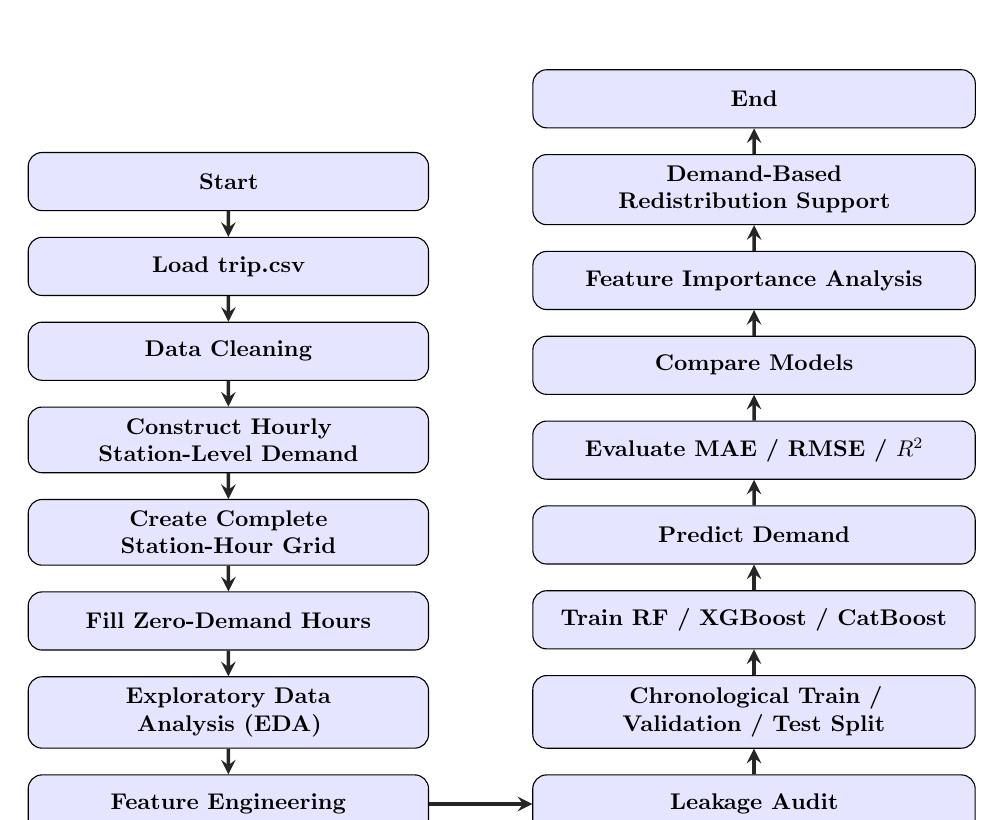
\begin{tikzpicture}[auto, scale=0.82, every node/.style={transform shape}]
    % Styles for left and right columns
    \tikzstyle{lproc} = [rectangle, minimum width=6.2cm, minimum height=0.9cm, align=center, text width=5.8cm, draw=black, fill=blue!10, font=\normalsize\bfseries, inner sep=5pt, rounded corners=5pt]
    \tikzstyle{rproc} = [rectangle, minimum width=6.8cm, minimum height=0.9cm, align=center, text width=6.5cm, draw=black, fill=blue!10, font=\normalsize\bfseries, inner sep=5pt, rounded corners=5pt]
    \tikzstyle{flowarrow} = [thick, ->, >=stealth, draw=black!85, line width=1.3pt]
    
    % LEFT COLUMN (Top to Bottom)
    \node [lproc] (start) {Start};
    \node [lproc, below=0.4cm of start] (step1) {Load trip.csv};
    \node [lproc, below=0.4cm of step1] (step2) {Data Cleaning};
    \node [lproc, below=0.4cm of step2] (step3) {Construct Hourly\\Station-Level Demand};
    \node [lproc, below=0.4cm of step3] (step4) {Create Complete\\Station-Hour Grid};
    \node [lproc, below=0.4cm of step4] (step5) {Fill Zero-Demand Hours};
    \node [lproc, below=0.4cm of step5] (step6) {Exploratory Data Analysis (EDA)};
    \node [lproc, below=0.4cm of step6] (step7) {Feature Engineering};
    
    % RIGHT COLUMN (Bottom to Top)
    \node [rproc, right=1.6cm of step7] (step8) {Leakage Audit};
    \node [rproc, above=0.4cm of step8] (step9) {Chronological Train /\\Validation / Test Split};
    \node [rproc, above=0.4cm of step9] (step10) {Train RF / XGBoost / CatBoost};
    \node [rproc, above=0.4cm of step10] (step11) {Predict Demand};
    \node [rproc, above=0.4cm of step11] (step12) {Evaluate MAE / RMSE / $R^2$};
    \node [rproc, above=0.4cm of step12] (step13) {Compare Models};
    \node [rproc, above=0.4cm of step13] (step14) {Feature Importance Analysis};
    \node [rproc, above=0.4cm of step14] (step15) {Demand-Based\\Redistribution Support};
    \node [rproc, above=0.4cm of step15] (end) {End};

    % Arrows Left (Downward)
    \draw [flowarrow] (start) -- (step1);
    \draw [flowarrow] (step1) -- (step2);
    \draw [flowarrow] (step2) -- (step3);
    \draw [flowarrow] (step3) -- (step4);
    \draw [flowarrow] (step4) -- (step5);
    \draw [flowarrow] (step5) -- (step6);
    \draw [flowarrow] (step6) -- (step7);
    
    % Arrow Bottom (Connect Left to Right across columns)
    \draw [flowarrow] (step7) -- (step8);
    
    % Arrows Right (Upward)
    \draw [flowarrow] (step8) -- (step9);
    \draw [flowarrow] (step9) -- (step10);
    \draw [flowarrow] (step10) -- (step11);
    \draw [flowarrow] (step11) -- (step12);
    \draw [flowarrow] (step12) -- (step13);
    \draw [flowarrow] (step13) -- (step14);
    \draw [flowarrow] (step14) -- (step15);
    \draw [flowarrow] (step15) -- (end);
\end{tikzpicture}
\caption{Activity Diagram of the Prediction Algorithm}
\label{fig:activity_diagram}

\end{figure}

This activity diagram outlines the end-to-end data processing and predictive modeling pipeline, mapping each logical step from raw data ingestion to the final redistribution support output:
\begin{itemize}\setlength{\itemsep}{2pt}\setlength{\parskip}{0pt}
    \item \textbf{Step 1 -- Load \texttt{trip.csv}:} Ingest 669,959 historical bicycle trip records containing timestamps and station identifiers.
    \pagebreak
    \item \textbf{Step 2 -- Data Cleaning:} Audit the trip records for missing values and invalid entries, and parse the timestamp fields into standardized datetime values.
    \item \textbf{Step 3 -- Construct Hourly Station Demand:} Group trip records by departure station and 1-hour intervals to compute hourly departure volumes.
    \item \textbf{Step 4 -- Create Complete Station-Hour Grid:} Cross-join all 70 docking stations with all 17,583 continuous timeline hours.
    \item \textbf{Step 5 -- Fill Zero-Demand Hours:} Explicitly assign a count of zero departures to inactive station-hours.
    \item \textbf{Step 6 -- Exploratory Data Analysis (EDA):} Uncover commuter rush-hour peaks, day-of-week trends, and high-traffic station hubs.
    \item \textbf{Step 7 -- Feature Engineering:} Compute 54 predictive features, including cyclic encodings, historical lags, and rolling metrics.
    \item \textbf{Step 8 -- Leakage Audit:} Strictly verify that all features utilize only information available prior to the forecast horizon.
    \item \textbf{Step 9 -- Chronological Split:} Partition records chronologically into Train (70\%, 861,560 rows), Validation (15\%, 184,590 rows), and Test (15\%, 184,660 rows) sets.
    \item \textbf{Step 10 -- Train RF / XGBoost / CatBoost:} Fit Random Forest, XGBoost, and CatBoost ensemble models on the training partition.
    \item \textbf{Step 11 -- Predict Demand:} Generate continuous departure predictions on unseen future test observations.
    \item \textbf{Step 12 -- Evaluate MAE / RMSE / $R^2$:} Quantify error magnitudes and explained variance across test predictions.
    \item \textbf{Step 13 -- Compare Models:} Objectively benchmark the three models on the authoritative test metrics.
    \item \textbf{Step 14 -- Feature Importance Analysis:} Analyze the relative mathematical contributions of engineered features.
    \item \textbf{Step 15 -- Demand-Based Redistribution Support:} Provide forecast outputs to assist transit operators in proactively rebalancing bicycles across stations.
\end{itemize}


The step-by-step working of the algorithm reflects a complete end-to-end regression pipeline, starting from raw transaction data ingestion to model evaluation and generating redistribution support, completely omitting forward-looking bias.

\needspace{10\baselineskip}
\textbf{1. Random Forest}

\begin{figure}[H]
\centering
\includegraphics[width=0.62\textwidth]{diagram_3.pdf}
\caption{Flow Chart for Random Forest Algorithm}
\label{fig:rf_flow}

\end{figure}

This architectural flow diagram illustrates the internal mechanics of the Random Forest algorithm:
\begin{itemize}
    \item \textbf{Step 1 -- Bootstrap Sampling:} Draw 200 independent random sample sets with replacement from the training data.
    \pagebreak
    \item \textbf{Step 2 -- Random Feature Subspace Selection:} At each split node, select a random subset of features ($\sqrt{m} \approx 7$ features) to decorrelate individual decision trees.
    \item \textbf{Step 3 -- Decision Tree Construction:} Train an individual decision tree on each bootstrap sample up to \texttt{max\_depth} = 15, with \texttt{min\_samples\_split} = 10 and \texttt{min\_samples\_leaf} = 2.
    \item \textbf{Step 4 -- Parallel Model Inference:} Pass the feature vector through all 200 trees simultaneously to produce individual continuous predictions.
    \item \textbf{Step 5 -- Ensemble Averaging:} Compute the arithmetic mean of all 200 independent tree outputs to produce the final continuous demand forecast.
\end{itemize}


The bimodal demand distribution, characterized by morning and evening commuter surges between transit hubs and commercial districts, causes structural inventory imbalances across the station network. Accurate hourly departure forecasting allows fleet operators to anticipate station deficits and capacity bottlenecks, supporting proactive, demand-based redistribution planning.

Random Forest addresses this forecasting task by constructing an ensemble of 200 de-correlated decision trees. To mitigate overfitting on historical training observations, the algorithm incorporates bootstrap aggregation (bagging) by fitting each tree on an independently drawn sample with replacement, while restricting split candidates to a random subset of features ($\sqrt{m} \approx 7$). The final station-hour departure prediction is obtained by computing the arithmetic mean across all 200 individual tree outputs, effectively reducing variance while maintaining robust generalization on tabular regression data.


\needspace{10\baselineskip}
\textbf{2. XGBoost (Extreme Gradient Boosting)}

\begin{figure}[H]
\centering
\includegraphics[width=0.70\textwidth]{diagram_4.pdf}
\caption{Flow Chart for XGBoost Algorithm}
\label{fig:xgb_flow}

\end{figure}

This diagram depicts the sequential architecture of XGBoost:
\begin{itemize}
    \pagebreak
    \item \textbf{Step 1 -- Data Ingestion \& Preprocessing:} Load and clean the station-hour dataset to prepare predictor features.
    \item \textbf{Step 2 -- Model Initialization \& Initial Prediction:} Initialize the XGBoost regressor and generate a baseline prediction across all instances.
    \item \textbf{Step 3 -- Decision Tree Construction:} Build a shallow regression tree (\texttt{max\_depth} = 10) on the engineered features.
    \item \textbf{Step 4 -- Prediction Error Calculation:} Calculate residual errors using first- and second-order loss gradients.
    \item \textbf{Step 5 -- Sequential Error Reduction (600 Rounds):} Iteratively construct subsequent trees to correct prior residual errors, repeating for 600 boosting rounds.
    \item \textbf{Step 6 -- Final Model Evaluation \& Forecasting:} Form the final ensemble, evaluate using MAE, RMSE, and $R^2$, and forecast hourly station-level departure demand.
\end{itemize}


While Random Forest builds hundreds of trees independently at the exact same time, XGBoost (Extreme Gradient Boosting) takes a completely different, sequential approach. XGBoost builds trees one by one, where every new tree is specifically designed to fix the mistakes made by the previous trees. 

Imagine a student taking a math test. A Random Forest is like 200 students taking the test independently and averaging their scores. XGBoost is like one student taking the test, seeing exactly which questions they got wrong, studying only those specific weak areas, and taking the test again, repeating this process sequentially to minimize residual errors across iterations. 

In the context of our bike-sharing dataset, the first XGBoost tree might make a rough guess. The model predicts 10 departures, while the actual observed demand was 15 departures. This means it was off by 5 (this mistake is called the residual error). The second tree is then built not to predict the total number of bicycles, but specifically to predict that missing value of 5. By continuously chaining these highly focused, corrective trees together, XGBoost iteratively reduces the residual error. 

XGBoost employs second-order Taylor expansions to optimize the loss function, utilizing both first- and second-order gradients to determine optimal tree splits. In addition, explicit $L_2$ regularization on leaf weights penalizes excessive model complexity. Through iterative tree construction and shrinkage ($\eta = 0.04$), XGBoost provides a structured, gradient-driven approach to regression on tabular data.



\needspace{10\baselineskip}
\textbf{3. CatBoost (Categorical Boosting)}

\begin{figure}[H]
\centering
\includegraphics[width=0.70\textwidth]{diagram_5.pdf}
\caption{Flow Chart for CatBoost Algorithm}
\label{fig:cat_flow}

\end{figure}

This flow diagram details CatBoost's generation of symmetric (oblivious) decision trees:
\begin{itemize}
    \item \textbf{Step 1 -- Ordered Permutation Setup:} Generate random permutations of the dataset to establish a strict temporal sequence.
    \item \textbf{Step 2 -- Ordered Target Statistics:} Compute statistics using only prior samples in the permutation, preventing target leakage.
    \item \textbf{Step 3 -- Symmetric Oblivious Tree Construction:} Build symmetric trees of depth 8 where every node at the same level shares identical split conditions.
    \item \textbf{Step 4 -- Regularized Loss Optimization:} Optimize leaf weights using RMSE loss with an $L_2$ leaf regularization coefficient of 3.
    \item \textbf{Step 5 -- Additive Model Aggregation:} Sum the predictions across all 600 symmetric trees to produce the final continuous demand forecast.
\end{itemize}


CatBoost, developed by Yandex, is another advanced gradient boosting algorithm similar to XGBoost, but it was specifically engineered to solve two major problems that plague traditional boosting models: target leakage and the handling of complex categories.

In traditional boosting, when a tree is trying to figure out how to correct an error, it looks at the target value of the exact data point it is trying to predict. This can lead to a phenomenon called "target leakage" or "prediction shift," where the model subtly cheats by relying on information it shouldn't have access to. If a model memorizes these leaked patterns, it will perform incredibly well on the training data but fail miserably when deployed in the real world. CatBoost solves this entirely by using a brilliant technique called "Ordered Boosting." It randomly shuffles the data and only allows the model to learn from historical rows that occurred *before* the current row in the permutation. This ensures that the algorithm learns patterns without target leakage rather than memorizing anomalies.

Furthermore, CatBoost builds "symmetric" or "oblivious" decision trees. In a standard decision tree, the left side of the tree might grow very deep while the right side stops early. In a CatBoost tree, every single node at the same depth is forced to use the exact same splitting rule. For example, if the tree decides to split based on "Is the hour > 12?" at depth 2, it applies that rule across the entire level. While this might sound restrictive, it acts as a massive safeguard against overfitting. It also facilitates computationally efficient inference. This structure supports practical prediction across multiple stations.

\needspace{12\baselineskip}
\subsection{Project pipeline}

\begin{figure}[H]
\centering
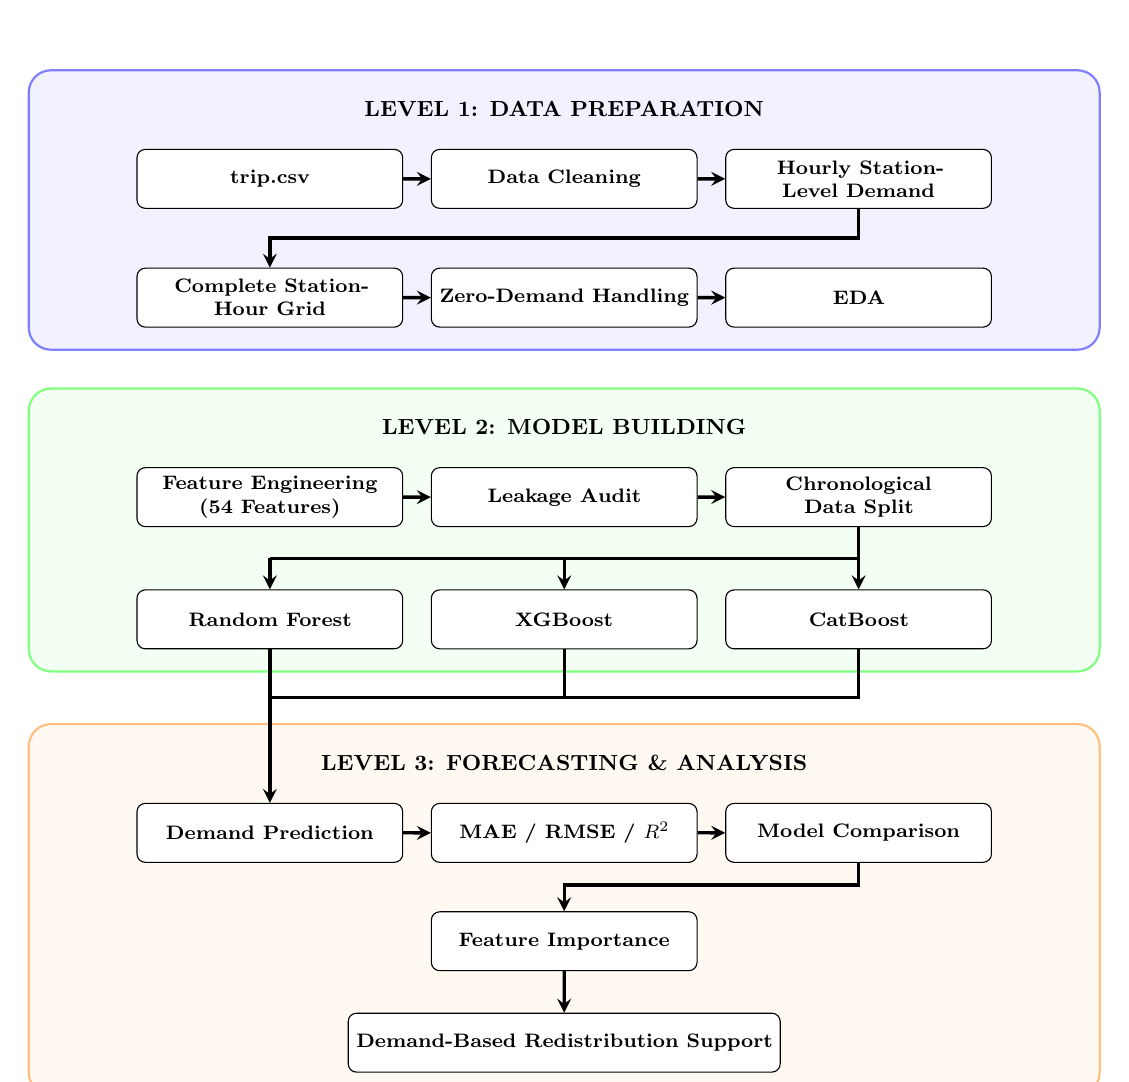
\begin{tikzpicture}[auto, scale=0.88, every node/.style={transform shape}]
    \pgfdeclarelayer{background}
    \pgfsetlayers{background,main}

    % Node styles
    \tikzstyle{mybox} = [rectangle, minimum width=3.8cm, minimum height=0.85cm, align=center, text width=3.6cm, draw=black, fill=white, font=\footnotesize\bfseries, rounded corners=3pt]
    \tikzstyle{widebox} = [rectangle, minimum width=3.8cm, minimum height=0.85cm, align=center, text width=3.6cm, draw=black, fill=white, font=\footnotesize\bfseries, rounded corners=3pt]
    \tikzstyle{bigbox} = [rectangle, minimum width=6.2cm, minimum height=0.85cm, align=center, text width=6.0cm, draw=black, fill=white, font=\footnotesize\bfseries, rounded corners=3pt]
    \tikzstyle{grouplabel} = [font=\small\bfseries, text=black]
    \tikzstyle{flowarrow} = [line width=1.2pt, ->, >=stealth, draw=black]
    \tikzstyle{busline} = [line width=1.2pt, draw=black]

    % =========================================================================
    % LEVEL 1: DATA PREPARATION
    % =========================================================================
    \node [grouplabel] (l1_title) at (0, 0) {LEVEL 1: DATA PREPARATION};
    
    \node [mybox, below=0.35cm of l1_title] (clean) {Data Cleaning};
    \node [mybox, left=0.4cm of clean] (csv) {trip.csv};
    \node [mybox, right=0.4cm of clean] (demand) {Hourly Station-Level Demand};
    
    \node [mybox, below=0.85cm of clean] (zero) {Zero-Demand Handling};
    \node [mybox, left=0.4cm of zero] (grid) {Complete Station-Hour Grid};
    \node [mybox, right=0.4cm of zero] (eda) {EDA};

    % =========================================================================
    % LEVEL 2: MODEL BUILDING
    % =========================================================================
    \node [grouplabel, below=1.2cm of zero] (l2_title) {LEVEL 2: MODEL BUILDING};
    
    \node [mybox, below=0.35cm of l2_title] (audit) {Leakage Audit};
    \node [mybox, left=0.4cm of audit] (feat) {Feature Engineering\\(54 Features)};
    \node [mybox, right=0.4cm of audit] (split) {Chronological Data Split};
    
    \node [mybox, below=0.9cm of audit] (xgb) {XGBoost};
    \node [mybox, left=0.4cm of xgb] (rf) {Random Forest};
    \node [mybox, right=0.4cm of xgb] (cat) {CatBoost};

    % =========================================================================
    % LEVEL 3: FORECASTING & ANALYSIS
    % =========================================================================
    \node [grouplabel, below=1.4cm of xgb] (l3_title) {LEVEL 3: FORECASTING \& ANALYSIS};
    
    \node [widebox, below=0.35cm of l3_title] (eval) {MAE / RMSE / $R^2$};
    \node [widebox, left=0.4cm of eval] (pred) {Demand Prediction};
    \node [widebox, right=0.4cm of eval] (comp) {Model Comparison};
    
    \node [widebox, below=0.7cm of eval] (imp) {Feature Importance};
    \node [bigbox, below=0.6cm of imp] (redist) {Demand-Based Redistribution Support};

    % =========================================================================
    % BACKGROUND CONTAINERS (Rendered behind all nodes and arrows)
    % =========================================================================
    \begin{pgfonlayer}{background}
        \node [rectangle, draw=blue!50, fill=blue!5, thick, rounded corners=8pt, minimum width=13.6cm, inner ysep=8pt, fit=(l1_title) (csv) (demand) (grid) (eda)] (box_l1) {};
        \node [rectangle, draw=green!50, fill=green!5, thick, rounded corners=8pt, minimum width=13.6cm, inner ysep=8pt, fit=(l2_title) (feat) (split) (rf) (cat)] (box_l2) {};
        \node [rectangle, draw=orange!50, fill=orange!5, thick, rounded corners=8pt, minimum width=13.6cm, inner ysep=8pt, fit=(l3_title) (pred) (comp) (imp) (redist)] (box_l3) {};
    \end{pgfonlayer}

    % =========================================================================
    % ARROWS AND FLOW CONNECTORS (Drawn on top layer for guaranteed visibility)
    % =========================================================================
    % Level 1 Flow
    \draw [flowarrow] (csv) -- (clean);
    \draw [flowarrow] (clean) -- (demand);
    \draw [flowarrow] (demand.south) -- ++(0,-0.42) -| (grid.north);
    \draw [flowarrow] (grid) -- (zero);
    \draw [flowarrow] (zero) -- (eda);

    % Level 2 Flow
    \draw [flowarrow] (feat) -- (audit);
    \draw [flowarrow] (audit) -- (split);
    
    % Level 2 Split to 3 Models
    \coordinate (split_bus) at ($(audit.south)!0.5!(xgb.north)$);
    \draw [busline] (split.south) |- (split_bus);
    \draw [busline] (rf.north |- split_bus) -- (cat.north |- split_bus);
    \draw [flowarrow] (rf.north |- split_bus) -- (rf.north);
    \draw [flowarrow] (xgb.north |- split_bus) -- (xgb.north);
    \draw [flowarrow] (cat.north |- split_bus) -- (cat.north);

    % Models to Demand Prediction (Collector bar beneath RF, XGBoost, CatBoost)
    \coordinate (col_bus) at ($(xgb.south)!0.5!(l3_title.north)$);
    \draw [busline] (rf.south) |- (col_bus);
    \draw [busline] (cat.south) |- (col_bus);
    \draw [busline] (xgb.south) -- (xgb.south |- col_bus);
    \draw [busline] (rf.south |- col_bus) -- (cat.south |- col_bus);
    \draw [flowarrow] (pred.north |- col_bus) -- (pred.north);

    % Level 3 Flow
    \draw [flowarrow] (pred) -- (eval);
    \draw [flowarrow] (eval) -- (comp);
    \draw [flowarrow] (comp.south) -- ++(0,-0.32) -| (imp.north);
    \draw [flowarrow] (imp) -- (redist);
\end{tikzpicture}
\caption{Project Workflow}
\label{fig:project_workflow}

\end{figure}

The project pipeline follows a structured three-tier architecture:
\begin{itemize}\setlength{\itemsep}{1pt}\setlength{\parskip}{0pt}
    \item \textbf{Level 1 -- Data Preparation:} The trip data is cleaned and aggregated into hourly station-level departure demand. A complete station-hour grid is constructed and zero-demand periods are represented explicitly before exploratory analysis.
    \item \textbf{Level 2 -- Model Building:} The prepared data is transformed into 54 engineered features, checked through a leakage audit, and divided chronologically into training, validation, and test sets. Random Forest, XGBoost, and CatBoost are trained independently.
    \item \textbf{Level 3 -- Forecasting and Analysis:} The trained models generate demand predictions for unseen data. Performance is evaluated using MAE, RMSE, and $R^2$, followed by model comparison and feature-importance analysis. The forecasts can support demand-based redistribution planning.
\end{itemize}


\subsection{Feasibility Analysis}

\noindent\textbf{Technical Feasibility:} The proposed system is technically feasible because it uses established Python libraries and machine-learning algorithms for tabular regression. The dataset can be processed on a standard computer, and the workflow includes data preprocessing, feature engineering, chronological splitting, model training, and evaluation using MAE, RMSE, and $R^2$. Random Forest, XGBoost, and CatBoost can be trained independently using the engineered station-hour dataset.

\vspace{0.5em}
\noindent\textbf{Economic Feasibility:} The project is economically feasible because the implementation uses open-source programming tools and machine-learning libraries. No specialized or expensive software infrastructure is required. The models can be developed and evaluated using a standard computer with sufficient memory and storage.

\vspace{0.5em}
\noindent\textbf{Operational Feasibility:} The system is operationally feasible because the predicted hourly station-level departure demand can support demand-based redistribution planning. The current implementation uses historical trip data and does not provide real-time bike availability or calculate the exact number of bicycles to be moved between stations.

\subsection{System Environment}

\subsubsection{Software Environment}
The project was developed using Python and commonly used data-science and machine-learning libraries. Pandas and NumPy were used for data processing and feature preparation. Scikit-learn was used for Random Forest and evaluation utilities, while XGBoost and CatBoost were used for gradient-boosting regression. Matplotlib and Seaborn were used for exploratory data analysis and visualization. Jupyter Notebook and VS Code were utilized as the primary interactive development environments.

\begin{itemize}\setlength{\itemsep}{1pt}\setlength{\parskip}{0pt}
    \item Python 3.10
    \item Pandas
    \item NumPy
    \item Scikit-learn
    \item XGBoost
    \item CatBoost
    \item Matplotlib
    \item Seaborn
\end{itemize}

\subsubsection{Hardware Environment}
The project was developed and executed on a standard personal computer suitable for data processing and machine-learning model training. A minimum configuration of an Intel Core i5 processor, 8 GB RAM, and approximately 5 GB of available storage is sufficient for the implementation, while 16 GB RAM is recommended for smoother processing of the complete station-hour dataset and model training.


% ==============================================================================
% 4. SYSTEM DESIGN
% ==============================================================================
\section{System Design}
\subsection{Models Building}

\subsubsection{Implementation code}

\begin{lstlisting}[
language=Python,
caption={Representative Model Implementation},
breaklines=true,
breakatwhitespace=false,
basicstyle=\small\ttfamily,
columns=fullflexible
]
import pandas as pd
from sklearn.ensemble import RandomForestRegressor
from xgboost import XGBRegressor
from catboost import CatBoostRegressor

df = pd.read_csv("station_hour_grid_engineered.csv")
df["timestamp"] = pd.to_datetime(df["timestamp"])

train_end = pd.to_datetime("2015-01-24 04:00:00")
val_end = pd.to_datetime("2015-05-14 01:00:00")

train_df = df[df["timestamp"] <= train_end]
val_df = df[(df["timestamp"] > train_end) &
            (df["timestamp"] <= val_end)]
test_df = df[df["timestamp"] > val_end]

X_train = train_df.drop(["demand", "timestamp"], axis=1)
y_train = train_df["demand"]

X_val = val_df.drop(["demand", "timestamp"], axis=1)
y_val = val_df["demand"]

X_test = test_df.drop(["demand", "timestamp"], axis=1)
y_test = test_df["demand"]

rf_model = RandomForestRegressor(
    n_estimators=200,
    max_depth=15,
    min_samples_split=10,
    min_samples_leaf=2,
    max_features="sqrt",
    random_state=42,
    n_jobs=-1
)

xgb_model = XGBRegressor(
    n_estimators=600,
    max_depth=10,
    learning_rate=0.04,
    subsample=0.8,
    colsample_bytree=0.8,
    min_child_weight=1,
    reg_alpha=0,
    reg_lambda=1,
    objective="reg:squarederror",
    eval_metric="rmse",
    random_state=42,
    n_jobs=-1
)

cat_model = CatBoostRegressor(
    iterations=600,
    depth=8,
    learning_rate=0.05,
    l2_leaf_reg=3,
    loss_function="RMSE",
    eval_metric="RMSE",
    random_seed=42,
    verbose=False,
    thread_count=-1
)

rf_model.fit(X_train, y_train)
xgb_model.fit(X_train, y_train)
cat_model.fit(X_train, y_train)
\end{lstlisting}

The implementation loads the prepared station-hour dataset, performs chronological partitioning into training, validation, and test sets, separates the target variable from the predictor variables, and independently trains the Random Forest, XGBoost, and CatBoost regression models. The complete model configurations, training times, and development metrics are presented in Section~4.1.3.

\needspace{12\baselineskip}
\subsubsection{Model Planning (Training/ Testing split of the dataset)}
\begin{figure}[H]
\centering
\includegraphics[width=0.9\textwidth]{fig_3_26_train_test_split.png}
\caption{Chronological Dataset Splitting}
\label{fig:train_test_split}

\end{figure}

This chronological visualization explicitly demonstrates how the grid was partitioned to prevent data leakage (70\% train, 15\% val, 15\% test) based strictly on time.


\subsubsection{Training}
The predictive models were trained to forecast hourly station-level departure demand across the network. Training was conducted using 861,560 chronological records covering the period from 29 August 2013 at 09:00:00 to 24 January 2015 at 04:00:00. Three ensemble regression algorithms were trained independently on this identical training set: Random Forest Regressor, Extreme Gradient Boosting (XGBoost) Regressor, and CatBoost Regressor.

The specific hyperparameter configurations defining the model implementations are as follows:

\begin{itemize}\sloppy\setlength{\itemsep}{2pt}\setlength{\parskip}{0pt}
    \item \textbf{Random Forest Regressor:}
    \texttt{n\_estimators} = 200, \texttt{max\_depth} = 15, \texttt{min\_samples\_split} = 10, \texttt{min\_samples\_leaf} = 2, \texttt{max\_features} = \texttt{sqrt}, \texttt{random\_state} = 42, \texttt{n\_jobs} = -1.
    \item \textbf{XGBoost Regressor:}
    \texttt{n\_estimators} = 600, \texttt{max\_depth} = 10, \texttt{learning\_rate} = 0.04, \texttt{subsample} = 0.8, \texttt{colsample\_bytree} = 0.8, \texttt{min\_child\_weight} = 1, \texttt{reg\_alpha} = 0, \texttt{reg\_lambda} = 1, \texttt{objective} = \texttt{reg:squarederror}, \texttt{eval\_metric} = \texttt{rmse},\linebreak \texttt{random\_state} = 42, \texttt{n\_jobs} = -1.
    \item \textbf{CatBoost Regressor:}
    \texttt{iterations} = 600, \texttt{depth} = 8, \texttt{learning\_rate} = 0.05, \texttt{l2\_leaf\_reg} = 3, \texttt{loss\_function} = \texttt{RMSE}, \texttt{eval\_metric} = \texttt{RMSE}, \texttt{random\_seed} = 42, \texttt{verbose} = False, \texttt{thread\_count} = -1.
\end{itemize}

The measured training duration for each independent model on the training data is recorded as:
\begin{itemize}
    \item \textbf{Random Forest:} 44.47 seconds
    \item \textbf{XGBoost:} 386.06 seconds
    \item \textbf{CatBoost:} 35.13 seconds
\end{itemize}

During model development, empirical performance metrics were tracked across both the training partition (861,560 records) and the contiguous validation partition (184,590 records, spanning 24 January 2015 05:00:00 to 14 May 2015 01:00:00) to examine model performance and learning behavior. The recorded metrics are summarized in Table~\ref{tab:training_validation_metrics}.

\begin{table}[H]
\centering
\renewcommand{\arraystretch}{1.3}
\begin{tabular}{|l|c|c|c|c|c|c|}
\hline
\textbf{Model} & \multicolumn{3}{c|}{\textbf{Training Metrics}} & \multicolumn{3}{c|}{\textbf{Validation Metrics}} \\ \cline{2-7} 
 & \textbf{MAE} & \textbf{RMSE} & \textbf{$R^2$} & \textbf{MAE} & \textbf{RMSE} & \textbf{$R^2$} \\ \hline
Random Forest & 0.372124 & 0.743818 & 0.738601 & 0.422730 & 0.893547 & 0.730307 \\ \hline
XGBoost & 0.326834 & 0.622357 & 0.817001 & 0.413841 & 0.886436 & 0.734582 \\ \hline
CatBoost & 0.396745 & 0.799422 & 0.698059 & 0.417276 & 0.883352 & 0.736426 \\ \hline
\end{tabular}
\caption{Training and Validation Performance Metrics Across Independent Models}
\label{tab:training_validation_metrics}
\end{table}

These training and validation metrics were observed during development to check convergence and model stability. Final model comparison and evaluation must strictly be based on the unseen test set presented in Section~4.1.4 and Section~5.

\subsubsection{Testing}
The generalization capability of the trained models was evaluated on a dedicated, previously unseen test dataset comprising 184,660 records. This test partition strictly covers the future chronological window from 14 May 2015 at 02:00:00 to 31 August 2015 at 23:00:00. Because this period follows both the training and validation horizons chronologically, none of these observations were utilized during model training or parameter tuning, thereby ensuring a rigorous and realistic simulation of prospective operational deployment.

Each model was deployed to predict the target variable, defined as the hourly station-level departure demand---representing the number of trips starting from a particular station during a particular hour. Model performance on these unseen observations was quantified using standard regression metrics: Mean Absolute Error (MAE), Root Mean Squared Error (RMSE), and the Coefficient of Determination ($R^2$).

The empirical test results across the three models are summarized in Table~\ref{tab:test_evaluation_summary}.

\begin{table}[H]
\centering
\renewcommand{\arraystretch}{1.3}
\begin{tabular}{|l|c|c|c|}
\hline
\textbf{Model} & \textbf{MAE} & \textbf{RMSE} & \textbf{$R^2$} \\ \hline
Random Forest & 0.439206 & 0.908465 & 0.731390 \\ \hline
XGBoost & 0.430550 & 0.898213 & 0.737418 \\ \hline
CatBoost & 0.436126 & 0.897665 & 0.737738 \\ \hline
\end{tabular}
\caption{Empirical Model Evaluation on Unseen Test Dataset ($N = 184,660$)}
\label{tab:test_evaluation_summary}
\end{table}

An objective analysis of these test results indicates that:
\begin{itemize}
    \item XGBoost achieved the lowest MAE ($0.430550$), indicating slightly smaller average absolute deviations on typical demand hours.
    \item CatBoost achieved the lowest RMSE ($0.897665$) and the highest $R^2$ ($0.737738$), demonstrating resilience against larger residual errors.
    \item XGBoost and CatBoost exhibited closely comparable test performance across all three evaluation metrics.
    \item Random Forest served as an effective baseline model, achieving an $R^2$ of $0.731390$.
\end{itemize}


% ==============================================================================
% 5. RESULTS AND DISCUSSION
% ==============================================================================
\section{Results and Discussion}
\subsection{Comparison of models}

\begin{figure}[H]
\centering
\textbf{Random Forest Verified Training Metrics:}
\begin{itemize}\setlength{\itemsep}{1pt}\setlength{\parskip}{0pt}
    \item Train MAE = 0.372124
    \item Train RMSE = 0.743818
    \item Train $R^2$ = 0.738601
\end{itemize}
\caption{Random Forest Evaluation Results}
\label{fig:rf_results}
\end{figure}

The validated metrics achieved by Random Forest during the training phase.

\begin{table}[H]
\centering
\renewcommand{\arraystretch}{1.2}
\begin{tabular}{|l|c|c|c|}
\hline
\textbf{Model} & \textbf{MAE} & \textbf{RMSE} & \textbf{$R^2$} \\ \hline
Random Forest & 0.439206 & 0.908465 & 0.731390 \\ \hline
XGBoost & 0.430550 & 0.898213 & 0.737418 \\ \hline
CatBoost & 0.436126 & 0.897665 & 0.737738 \\ \hline
\end{tabular}
\caption{Final Testing Set Results and Model Comparison ($N = 184,660$)}
\label{tab:model_comparison}
\end{table}

\subsection{Evaluation metrics}
MAE (Mean Absolute Error) measures average magnitude of errors. RMSE (Root Mean Squared Error) heavily penalizes large errors. $R^2$ indicates the proportion of variance explained by the model.

\subsection{Confusion Matrix}
Confusion matrices are primarily used for classification problems. Since the proposed system predicts numerical hourly demand, the implemented task is regression and a confusion matrix is therefore not applicable to the primary model evaluation.

\subsection{Relevant Metrics Calculated from Confusion Matrix}
Precision, recall and F1-score are classification metrics and are therefore not used for the primary evaluation of this regression problem. MAE, RMSE and $R^2$ are used for evaluating the demand predictions.

\clearpage
\subsection{Prediction statistics of unseen data}
The final evaluation was performed on 184,660 unseen observations representing chronological data from 14 May 2015 to 31 August 2015. 

\begin{figure}[H]
\centering
\includegraphics[width=0.70\textwidth]{actual_vs_predicted_catboost.png}
\caption{Actual vs Predicted Hourly Demand}
\label{fig:actual_vs_predicted}
\end{figure}

This visualization demonstrates the model's performance on unseen chronological test data. It contrasts the model's regression output against actual observed departure demands.

\begin{figure}[H]
\centering
\includegraphics[width=0.72\textwidth]{fig_5_4_prediction_result.png}
\caption{Prediction Result Statistics}
\label{fig:prediction_result}
\end{figure}

This screenshot displays empirical prediction metrics obtained across test observations.

\clearpage
\subsection{Findings and Conclusions}

The empirical investigation in this project was conducted using exclusively \texttt{trip.csv} from the SF Bay Area Bike Share Dataset, comprising 669,959 raw trip records across 70 start stations. The prediction target was formulated as hourly station-level departure demand, defined as: ``The number of trips starting from a particular station during a particular hour.'' To account for periods without trip initiations, a complete station-hour grid of 1,230,810 records was constructed, and zero-demand station-hours were retained as meaningful observations to maintain historical consistency across all stations and hours.

Exploratory data analysis identified pronounced temporal variations across the network. System-wide usage peaked during morning commuting periods, where 08:00 was the highest overall demand hour with 85,864 trips. Furthermore, Weekday demand was substantially higher than weekend demand, reflecting recurrent commuter travel routines rather than leisure activity. Substantial spatial concentration was also observed across individual docking locations; San Francisco Caltrain (Townsend at 4th) recorded the highest observed start-station demand with 49,092 trips, highlighting heavy departures at key transit interchanges. These patterns describe empirical historical associations without asserting causal mechanisms.

Following feature generation, 54 final features were engineered and audited to capture temporal calendar signals, cyclic rhythms, historical lags, and rolling statistical windows. A formal leakage audit did not detect target/current/future demand leakage. Model training and evaluation strictly adhered to chronological splitting to replicate real-world deployment, allocating 861,560 records for training, 184,590 records for validation, and 184,660 records for testing. The test set was an unseen future chronological period. Random Forest, XGBoost, and CatBoost were trained independently. Random Forest served as the baseline model. On the unseen test partition, Random Forest achieved an MAE of 0.439206, an RMSE of 0.908465, and an $R^2$ of 0.731390. XGBoost yielded an MAE of 0.430550, an RMSE of 0.898213, and an $R^2$ of 0.737418. CatBoost recorded an MAE of 0.436126, an RMSE of 0.897665, and an $R^2$ of 0.737738. XGBoost achieved the lowest MAE, while CatBoost achieved the lowest RMSE and highest $R^2$. The three models showed closely comparable performance.

In conclusion, the project developed a machine-learning pipeline for hourly station-level departure demand forecasting using historical trip data. By structuring transactional records into a complete station-hour grid and extracting leakage-free temporal and lag indicators, the generated forecasts provide demand-based redistribution support and forecast-driven redistribution planning for transit operators. Clearly, the current project does not calculate the exact number of physical bicycles to move because real-time bike availability is not available in \texttt{trip.csv}. Nonetheless, accurate hourly departure forecasting provides practical operational insights to anticipate station demand surges across the transit network.

\end{document}
